
\subparagraph{Spira circolare}
Si consideri una spira percorsa da corrente, disposta in modo simmetrico
rispetto all'asse $z$ e con centro coincidente con l'origine del sistema 
di riferimento. La distribuzione di corrente è simmetrica di rotazione quindi ci si 
aspetta che lo sia anche il campo di induzione magnetica rispetti la simmetria ossia
che sia indipendente dalla variabile azimutale $\varphi$.
\begin{figure}[H]
\centering
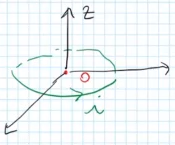
\includegraphics[width = 0.3\linewidth]{spira_circolare_magnetostatica}
\end{figure}
Applicando la legge di Ampere-Maxwell ad una curva di centro l'origine e raggio $r\neq R$
si ha che le componenti del campo $B_r$ e $B_\varphi$ godono della simmetria dispari.

Osservando invece la spira che giace sul piano $(r,y)$ si vedrebbe la corrente percorrere
la spira in un solo verso mentre una rotazione di $\pi$ attorno l'asse $r$ invertirebbe
il verso di percorrenza della corrente, si sta cioè osservando l'altro ``lato'' della spira.
Se oltre alla rotazione si cambia il segno della corrente e delle componenti del campo
allora la componente $B_r$ sarà in verso opposto rispetto al caso iniziale mentre
la componente $B_z$ ha conservato il proprio verso.
Si può concludere affermando che la simmetria di $B_r$ è pari mentre quella di $B_z$ è
dispari.

\subparagraph{Solenoide toroidale}
Sia l'asse $z$ l'asse di rotazione di una geometria piana cava qualsiasi che non intersechi
l'asse stesso. Il baricentro di questa geometria descrive una circonferenza di raggio $r$
mentre l'intera rotazione forma un toroide cavo con sezione costante.
\begin{figure}[H]
\centering
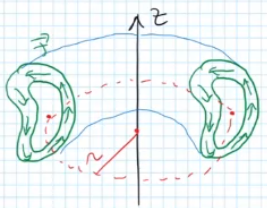
\includegraphics[width = 0.3\linewidth]{toroide_magnetostatica}
\end{figure}
La corrente $\vec{J}$ giace nei piani meridiani del fascio di asse $z$.
La simmetria della distribuzione rispetto a $\varphi$ implica che il campo è funzione solo
di $r$ e $z$.
$$
\vec{B} = \vec{B}(r,z) = B_r(r,z)\vec{e}_r + B_\varphi(r,z)\vec{e}_\varphi + B_z(r,z)\vec{e}_z 
$$

La componente $B_\varphi$ si calcola considerando linee circolari di centro l'asse $z$
e raggio $r$

Effettuando la circuitazione lungo $\Gamma$
$$
\oint_\Gamma \vec{B} \cdot \hat{t} dl = \mu_0 i_\Gamma = 2\pi r B_\varphi (r,z)  = \mu_0 N\cdot i
$$
dove $N$ è il numero di spire concatenate e $i$ la corrente che attraversa ciascuna spira.
Si ricava quindi che 
$$
B_\varphi (r,z) = \mu_0 \frac{Ni}{2\pi r}
$$
se $(r,z)$ è un punto interno al toroide.

Per analizzare le altre due componenti si ipotizza di avere un campo ipotetico
$$
\vec{B}^* = \vec{B} - B_\varphi(r,z)\vec{e}_\varphi
$$
che ha solo componenti $z$ ed $r$, giace quindi in ciascun piano meridiano di asse $z$
e soddisfa le equazioni di Maxwell omogenee, ossia non concatena alcuna corrente (perché interna
al piano stesso). È inoltre normale all'infinito dato che la distribuzione di corrente è al finito.
Per il teorema di Helmholtz se tutti i flussi e le circuitazioni sono pari a zero
e il campo è normale all'infinito, allora il campo $\vec{B}^*$ sarà proprio uguale a zero ossia
le componenti $B_r$ e $B_z$ sono pari a zero.

\subparagraph{Solenoide rettilineo indefinito}
Orientato un cilindro cavo lungo l'asse $z$ di spessore $\Delta$ in cui circola una corrente
$\vec{J}$ che giace nei piani perpendicolari a $z$ ed è simmetrica di rotazione rispetto a
$z$. Il solenoide rettilineo indefinito può essere visto come il limite per $r\to\infty$ del
solenoide toroidale. Il campo $\vec{B}$ sarà quindi diverso da zero anche in questo caso
solo all'interno del solenoide.
\begin{figure}[H]
\centering
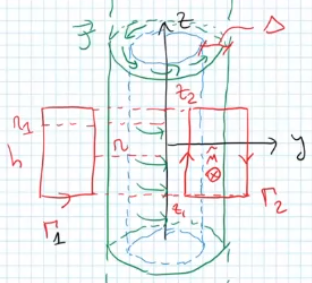
\includegraphics[width = 0.3\linewidth]{solenoide_indefinito_magnetostatica}
\end{figure}
Si prenda ora una linea $\Gamma_1$ esterna al solenoide e si esegua la circuitazione del campo
$$
\Gamma_1 : \oint_{\Gamma_1} \vec{B}\cdot\hat{t} dl = 0 \Rightarrow  \int_{z_1}^{z_1+h}B_z (r,z) - B_z(r_1,z)dz = 0
$$

Si prende invece un'altra linea $\Gamma_2$ con un lato interno al solenoide
$$
\Gamma_2 : \oint_{\Gamma_2} \vec{B}\cdot\hat{t}dl = \mu_0 h \Delta J = B_z(r,z) \cancel{h} =\mu_0\cancel{h}\Delta J
$$
Si definisce poi il numero di spire per unità di lunghezza $n=N/h$, la corrente di una spira è sempre $i$
quindi $Ni = nih = J\Delta h$ e l'espressione del campo diventa 
$$
\vec{B}(r,z) = 
\begin{cases}
\mu_0 n i \vec{e}_z & (r,z) \text{ interno al cilindro}\\
0 & \text{altrimenti}
\end{cases}
$$
Se si considera una superficie che attraversa il solenoide indefinito attraverso una sua sezione piena
si vedrà che il capo ha un andamento lineare decrescente tra la superficie interna ed esterna del solenoide
da $\mu_0 n i$ a zero.

\subsection{Magnetostatica nel vuoto in forma locale}
Si consideri un punto $P$ nel dominio $\Omega$, centro di un cubetto $\Delta\Omega$, allora
$$
\begin{aligned}
&\begin{cases}
\nabla\cdot\vec{B} &= 0\\
\nabla\times\vec{B} &= \mu_0\vec{J}
\end{cases} \text{ in }\Omega \text{ nei punti } P \text{ regolari} \\
&\hat{n}\cdot(\vec{B}_2-\vec{B}_1) = 0\\
&\hat{n}\times(\vec{B_2}-\vec{B}_1) = \mu_0 \vec{J}_s
\end{aligned}
$$

Se il dominio $\Omega$ è a connessione superficiale semplice il campo $\vec{B}$ è solenoidale
perché indivergente. Allora esso si potrà esprimere come il rotore di un altro campo vettoriale
$$
\vec{B} = \nabla\times\vec{A}
$$
$\vec{A}$ viene chiamato potenziale vettore magnetico, analogo al potenziale elettrico, solo che quello
di $\vec{E}$ è un potenziale scalare mentre quello appena definito è un potenziale vettore.

Per dimostrare l'equazione di Gauss si sfrutta il campo potenziale appena ricavato ricordando che la divergenza 
di un rotore è nulla.
$$
\nabla\cdot\vec{B} = 0 \Rightarrow \nabla\cdot(\nabla\times\vec{A}) = 0\ \forall\ \vec{A}
$$

Sia consideri l'equazione di Ampére-Maxwell in forma locale
$$
\nabla\times\vec{B} = \mu_0 \vec{J} = \nabla\times\nabla\times\vec{A} =  
\nabla(\nabla\cdot\vec{A}) - \nabla^2\vec{A} = \mu_0\vec{J}
$$

Per definire interamente un campo vettoriale è necessario determinarne sia divergenza che rotore, il 
rotore è stato ricavato, per la divergenza si esegue una scelta detta \textit{``della GAUGE''}, ossia
si sceglie un potenziale vettore arbitrario che abbia proprio divergenza nulla che viene detta
\textit{gauge di Coulomb}.
Se $\nabla\cdot\vec{A}=0$
$$
-\nabla^2\vec{A} = \mu_0\vec{J} = \begin{cases}
\nabla^2 A_x = -\mu_0 J_x \\
\nabla^2 A_y = -\mu_0 J_y \\
\nabla^2 A_z = -\mu_0 J_z 
\end{cases}
$$
Quella ottenuta viene definita equazione di Poisson vettoriale, fornita da tre equazioni
scalari.

Nel caso dell'elettrostatica si ha il potenziale di Coulomb:
$$
\nabla^2V = -\frac{\rho}{\varepsilon_0} \Rightarrow V(P) = \frac{1}{4\pi\varepsilon_0}\iiint_\Omega\frac{\rho(p')}{|\vec{r}_{p}-\vec{r}_{p'}|}dV
$$
In analogia matematica con il caso precedente il potenziale vettore del campo magnetico nel 
punto $P$
$$
\nabla^2\vec{A} = -\mu_0\vec{J} \Rightarrow \vec{A}(P) = \frac{\mu_0}{4\pi} \iiint_\Omega \frac{\vec{J}(p')}{|\vec{r}_p-\vec{r}_{p'}|}dV
$$
$\vec{A}(P)$ è il potenziale vettore prodotto in qualsiasi punto dello spazio dalla 
distribuzione di corrente $\vec{J}$ nel dominio $\Omega$.

Si consideri invece un potenziale vettore differente
$$
\vec{A}^*(P) = \vec{A} + \nabla\psi 
$$
Eseguendo il rotore si vede che esso è pari al rotore di $\vec{A}$ perché il rotore di un 
gradiente è sempre zero
$$
\nabla\times\vec{A}^* = \nabla\times\vec{A} + \cancel{\nabla\times\nabla\psi}
$$
Tutti i campi potenziali vettori a meno di un campo gradiente producono lo stesso
campo di induzione magnetica $\vec{B}$ nonostante sia differente invece la divergenza
del campo.
$$
\nabla\cdot\vec{A}^* = \nabla^2\psi
$$

\subsection{Legge di Biot-Savart}
Il campo $\vec{B}(P)$ si ricava con
$$
\vec{B}(P) = \nabla_p\times\vec{A} = \nabla_p \times \frac{\mu_0}{4\pi}\iiint_\Omega\frac{\vec{J}(p')}{|\vec{r}_p-\vec{r}_{p'}|}dV
$$
dove il pedice dell'operatore nabla specifica il punto rispetto a cui si eseguono le 
derivate.
Considerata la linearità degli operatori e che la derivata rispetto a $p$ non coinvolge
l'integrale è possibile invertire i termini
$$
\nabla_p\times\vec{A} = \frac{\mu_0}{4\pi}\iiint_\Omega \nabla_p\times\left(\frac{\vec{J}(p')}{|\vec{r}_p-\vec{r}_{p'}|}\right)dV
$$
ricordando l'identità vettoriale $\nabla\times(f\vec{v}) = f\nabla\times\vec{v} + \nabla f\times\vec{v}$  
\begin{align*}
f &= \frac{1}{|\vec{r}_p-\vec{r}_{p'}|} \\
\vec{v} &= \vec{J}(p')
\end{align*}
sostituendo e ricordando che il rotore rispetto a $p$ di una funzione
di $p'$ è nullo, come eseguire la derivata di una costante. Si ottiene
$$
\vec{B}(p) = \frac{\mu_0}{4\pi}\iiint_\Omega \nabla_p \left(\frac{1}{|\vec{r}_p-\vec{r}_{p'}|}\right) \times \vec{J}(p') dV
$$
Il prodotto vettoriale è antisimmetrico
$$
\vec{B}(p) = -\frac{\mu_0}{4\pi}\iiint_\Omega \vec{J}(p') \times\nabla_p\left(\frac{1}{|\vec{r}_p - \vec{r}_{p'}|}\right)dV
$$
Si ricorda inoltre che la \href{https://www.youmath.it/domande-a-risposte/view/5914-derivata-del-modulo.html}{derivata del valore assoluto} è la derivata di una funzione 
composta quindi il segno cambia se si deriva rispetto a $p$ o $p'$
$$
\nabla_p \left(\frac{1}{|\vec{r}_p - \vec{r}_{p'}|}\right) = -\nabla_{p'} \left(\frac{1}{|\vec{r}_p - \vec{r}_{p'}|}\right)
$$
Cambiando il segno
$$
\vec{B}(p) = \frac{\mu_0}{4\pi}\iiint_\Omega \vec{J}(p') \times\nabla_{p'}\left(\frac{1}{|\vec{r}_p - \vec{r}_{p'}|}\right)dV
$$
L'equazione appena ricavata è la \textit{Legge di Biot-Savart} e afferma che conoscendo
la densità di corrente, è possibile calcolare il campo $\vec{B}$ in tutto lo spazio
mediante un integrale.
Eseguendo anche il gradiente si può semplificare
$$
\vec{B}(p) = \frac{\mu_0}{4\pi}\iiint_\Omega \vec{J}(p') \times \frac{\vec{r}_p-\vec{r}_{p'}}{|\vec{r}_p - \vec{r}_{p'}|^3}dV
$$
\subparagraph{Analisi corrente quasi-filiforme}
Sia data una corrente in un circuito chiuso di sezione $S$ attraversato da una corrente
$i$, la densità di corrente sarà
$$
\vec{J}(p') = \frac{i}{S} \hat{t}(p')
$$
dove $\hat{t}(p')$ è il versore tangente alla linea media del circuito nel punto $p'$ 
identico al versore normale alla sezione trasversa.
$$
\vec{B}(p) = \frac{\mu_0}{4\pi}\oint_\Gamma \frac{i}{\cancel{S}}\hat{t}(p')\times\frac{\vec{r}_p-\vec{r}_{p'}}{|\vec{r}_p-\vec{r}_{p'}|^3} \cancel{S}dl
$$
$$
\vec{B}(p) = \frac{\mu_0}{4 \pi} i \oint_\Gamma \hat{t}(p') \times \frac{\vec{r}_p-\vec{r}_{p'}}{|\vec{r}_p-\vec{r}_{p'}|^3} dl
$$
Anche se non si riesce a calcolare l'integrale a causa di una difficile geometria
è possibile risolvere il problema numericamente con questa formula.
La funzione integranda
$$
d\vec{B} = \frac{\mu_0}{4\pi} i dl \times \frac{\vec{r}_p - \vec{r}_{p'}}{|\vec{r}_p - \vec{r}_{p'}|^3}
$$
rappresenta il contributo di campo infinitesimo del tratto elementare di corrente $idl$
anche se non ha un vero significato fisico, non ha senso considerare un tratto infinitesimo
di corrente se questa necessita di una linea chiusa in condizioni stazionarie per poter 
circolare. La precedente relazione prende in ogni caso il nome di 
\textit{Legge elementare di Laplace} ed è comunque utile a calcolare le distribuzioni
di campo.

\subparagraph{Campo di una spira circolare piana}
Sia una spira circolare piana $\Gamma$ di raggio $R$, il campo potenziale vettore
$$
\vec{A}(p) = \frac{\mu_0}{4\pi} \oint_\Gamma i \frac{\hat{t}(p')}{|\vec{r}_p - \vec{r}_{p'}|}dl
$$
\begin{align*}
\hat{t}(p') &= \vec{e}_\varphi' (R,\varphi',z'=0) \\
dl &= R d\varphi'\\
\vec{r}_{p'} & = r_{p'} \vec{e}_{r'} (R,\varphi',z'=0)
\end{align*}
\begin{figure}[H]
\centering
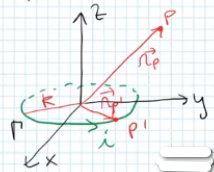
\includegraphics[width = 0.3\linewidth]{campo_A_spira_circolare}
\end{figure}
Sostituendo
$$
\vec{A}(p) = \frac{\mu_0 i}{4\pi}\oint_\Gamma \frac{R \vec{e}_\varphi (R,\varphi',z'=0)}{|r_p\vec{e}_r(r,\varphi,z)-r_{p'}\vec{e}_{r'}(R,\varphi',z'=0)|}d\varphi'
$$
Questa funzione può essere risolta analiticamente mediante gli integrali ellittici
ma è interessante prevalentemente valutare il campo a grande distanza $r_p >> r_{p'}$,
si approssima quindi la funzione
$$
\frac{1}{|\vec{r}_p-\vec{r}_{p'} |} = \left(r_p^2 + r_{p'}^2 - 2\vec{r}_p\cdot\vec{r}_{p'}\right)^{-\frac{1}{2}} = \frac{1}{r_p}\left(1+\left(\frac{r_{p'}}{r_p}\right)^2 - 2\frac{\vec{e}_r\cdot\vec{e}_{r'}}{r_p}r_{p'}\right)^{-\frac{1}{2}}
$$
Introducendo la variabile $\varepsilon=\frac{r_{p'}}{r_p}$
$$
\frac{1}{|\vec{r}_p-\vec{r}_{p'} |} = \frac{1}{r_p}\left(1 +\varepsilon^2 - 2A\varepsilon\right)^{-\frac{1}{2}}
$$
Dove la costante $A = \frac{\vec{e}_r\cdot\vec{e}_{r'}}{r_p}$.
Sviluppando in serie di Taylor al primo ordine e trascurando dunque $\varepsilon^2$ si 
ricorda che $\frac{1}{\sqrt{1+x}}\simeq 1 -\frac{x}{2} $ quindi l'equazione diventa
$$
\frac{1}{r_p}\left(1 +\cancel{\varepsilon^2} - 2A\varepsilon\right)^{-\frac{1}{2}} \simeq \frac{1}{r_p}\left(1+\frac{\vec{e}_r\cdot\vec{e}_{r'}}{r_p}r_{p'}\right) 
$$
Si conclude che a grande distanza ossia $r_p >> r_{p'}$
$$
\frac{1}{|\vec{r}_p-\vec{r}_{p'}|} \simeq \frac{1}{r_p} \left(1 + \frac{\vec{e}_r\cdot\vec{e}_{r'}}{r_p}r_{p'}\right)
$$
L'equazione semplificata del campo potenziale, ricordando che  $\hat{t}dl = Rd\vec{e}_{r'}$, diventa
$$
\vec{A}(p) = \frac{\mu_0 i}{4\pi}\oint_\Gamma \frac{R\ d\vec{e}_{r'}}{r_p} \left(1 + \frac{\vec{e}_r\cdot\vec{e}_{r'}}{r_p}r_{p'}\right) = \frac{\mu_0 i}{4\pi}\left[ \oint_\Gamma \frac{R\ d\vec{e}_{r'}}{r_p} + \oint_\gamma \frac{R^2}{r_p^2}(\vec{e}_r\cdot\vec{e}_{r'})d\vec{e}_{r'}\right]
$$
poiché $r_{p'} = R$. Il primo integrale è nullo perché è l'integrale del raggio vettore
su una circonferenza equivale alla somma dell'area positiva della semicirconferenza 
positiva e quella negativa della semicirconferenza inferiore.

In conclusione 
$$
\vec{A}(p) = \frac{\mu_0}{4\pi}iR^2 \oint_\Gamma \frac{(\vec{e}_r\cdot\vec{e}_{r'})}{r_p^2}d\vec{e}_{r'}
$$
Per svolgere l'integrale è necessario il seguente ``trucco'' algebrico, chiamato
dagli americani ``BAC-CAB''
\begin{align*}
\vec{a} &\times\left(\vec{b}\times\vec{c}\right) = \vec{b}\left(\vec{a}\cdot\vec{c}\right) - \vec{c}\left(\vec{a}\cdot\vec{b}\right) \\
\vec{e}_r &\times \left(\vec{e}_{r'}\times d\vec{e}_{r'}\right) = \vec{e}_{r'}\left(\vec{e}_r\cdot d\vec{e}_{r'}\right) - d\vec{e}_{r'}\left(\vec{e}_r\cdot\vec{e}_{r'}\right)
\end{align*}
Si analizza inoltre la seguente relazione
$$
d\varphi'\left(\vec{e}_{r'}\left(\vec{e}_r\cdot\vec{e}_{r'}\right)\right) = d\vec{e}_{r'} 
$$
1:42:20
